\ifx\wholebook\relax \else

\documentclass[b5paper]{article}
\usepackage[nomarginpar
  %, margin=.5in
]{geometry}

\addtolength{\oddsidemargin}{-0.05in}
\addtolength{\evensidemargin}{-0.05in}
\addtolength{\textwidth}{0.1in}

\usepackage[en]{../../../prelude}

\setcounter{page}{1}

\begin{document}

\title{List}

\author{Xinyu~LIU
\thanks{{\bfseries Xinyu LIU} \newline
  Email: liuxinyu95@gmail.com \newline}
  }

\maketitle
\fi

\markboth{List}{Elementary Algorithms}

\ifx\wholebook\relax
\chapter{List}
\numberwithin{Exercise}{chapter}
\fi

\section{Introduction}
\label{introduction}

List and array are build blocks for other complex data structure. Both hold multiple elements as a container. Array is a range of consecutive cells indexed by a number (address). It is typically bounded with fixed size. While list increases on-demand. One can traverse a list one by one from head to tail. Particularly in functional settings, list plays critical role to control the computation and logic flow\footnote{In low level, lambda calculus plays the most critical role as one of the computation model equivalent to Turing machine\cite{mittype}, \cite{unplugged}.}. Readers already be familiar with map, filter, fold are safe to skip this chapter, and directly start from chapter 2.

\section{Definition}
\index{List!definition}

List, or singly linked-list is a data structure recursively defined as: A {\em list} is either empty, denoted as $[\ ]$ or NIL; or contains an element and liked with a {\em list}. Figure \ref{fig:list-example} shows a list of nodes. Each contains two parts, an element (key), and a reference to the sub-list (next). The next to the last node is empty (NIL).

\begin{figure}[htbp]
  \centering
    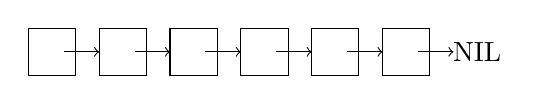
\begin{tikzpicture}[scale=3]
    \foreach \x in {-2, -1.7, ..., -0.4} {
      \draw (\x cm, 1cm) +(-0.1, -0.1) rectangle ++(0.1, 0.1);
      \draw[->] (\x cm, 1cm) +(0.05, 0) -- +(0.2, 0);
    }
    \draw (-0.2cm, 1cm) node {NIL};
    \end{tikzpicture}
  \caption{A list of nodes}
  \label{fig:list-example}
\end{figure}

Every node links to the next or NIL. We often define list with the compound structure\footnote{In most cases, the data stored in list have the same type. However, there is also heterogeneous list, like the list in Lisp for example.}, for example:

\lstset{frame=single}
\begin{lstlisting}[language=Bourbaki]
data List<A> {
    A key
    List<A> next
}
\end{lstlisting}

\index{List!empty} \index{List!empty testing}
Many traditional environments support the NIL concept. There are two ways to represent the empty list: one is to use NIL (or null, or $\nil$) directly; the other is to create a list, but put nothing as $[\ ]$. From implementation perspective, NIL need not allocate any memories, while $[\ ]$ does.

\subsection{Access}
\index{List!head} \index{List!tail} \index{List!Construction} \index{List!cons}
Given a none empty list $X$, define two functions\footnote{We often write function $f(x)$ as $f\ x$, and $f(x, y, ..., z)$ as $f\ x\ y\ ...\ z$.} to access the first element, and the rest sub-list. They are often called as \textit{first}\ $X$ and \textit{rest}\ $X$, or $head\ X$ and $tail\ X$\footnote{They are named as \texttt{car} and \texttt{cdr} in Lisp due to the design of machine registers\cite{SICP}.}. Conversely, we can construct a list from an element $x$ and another list $xs$ (can be empty), as $x \cons xs$. It is called the \texttt{cons} operation. We have the following equations:

\be
\begin{cases}
head\ (x \cons xs) & = x \\
tail\ (x \cons xs) & = xs
\end{cases}
\label{eq:list-head-tail}
\ee

For a none empty list $X$, we also denote the first element as $x_1$, and the rest sub-list as $X'$. For example, when $X = [x_1, x_2, x_3, ...]$, then $X' = [x_2, x_3, ...]$.

\begin{Exercise}
\Question{For list of type $A$, suppose we can test if any two elements $x, y \in A$ are equal, define an algorithm to test if two lists are identical.}
\end{Exercise}

\section{Basic operations}
\index{List!length}
From the definition, we can count the length recursively. the length of the empty list is 0, or it is 1 plus the length of the sub-list.

\be
\begin{array}{rcl}
length\ [\ ] & = & 0 \\
length\ (x \cons xs) & = & 1 + length\ xs
\end{array}
\ee

We traverse the list to count the length, the performance is bound to $O(n)$, where $n$ is the number of elements. We use $|X|$ as the length of $X$ when the context is clear. To avoid repeatedly counting, we can persist the length in a variable, and update it when mutate (add or delete). Below is the iterative length counting:

\begin{algorithmic}[1]
\Function{Length}{X}
  \State $n \gets 0$
  \While{$X \neq $ NIL}
    \State $n \gets n + 1$
    \State $X \gets $ \Call{Next}{$X$}
  \EndWhile
  \State \Return $n$
\EndFunction
\end{algorithmic}

\subsection{index}
\index{List!index} \index{List!get at}
Array supports random access at position $i$ in constant time, while we need traverse the list $i$ steps to access the target element.

\be
getAt\ i\ (x \cons xs) = \begin{cases}
  i = 0: & x \\
  i \neq 0: & getAt\ (i - 1)\ xs \\
\end{cases}
\ee

We leave the empty list not handled. The behavior when $[\ ]$ is undefined. As such, the out of bound case also leads to the undefined behavior. If $i > |X|$, we end up the edge case to access the $(i-|X|)$ position of the empty list. On the other hand, if $i < 0$, after minus it by one, it's even farther away from 0, and finally ends up with some negative position of the empty list. $getAt$ is bound to $O(i)$ time as it advances the list $i$ steps. Below is the imperative implementation:

\begin{algorithmic}[1]
\Function{Get-At}{$i, X$}
  \While{$i \neq 0$}
    \State $X \gets $ \Call{Next}{$X$}  \Comment{error when $X$ = NIL}
    \State $i \gets i - 1$
  \EndWhile
  \State \Return \Call{First}{$X$}
\EndFunction
\end{algorithmic}

\begin{Exercise}
\Question{In the iterative \textproc{Get-At}($i, X$) implementation, what is the behavior when $X$ is empty? what if $i$ is out of the bound or negative?}
\end{Exercise}

\subsection{Last}
\index{List!last} \index{List!init}

There is a pair of symmetric operations to `first/rest', namely `last/init'. For a none empty list $X = [x_1, x_2, ..., x_n]$, function $last$ returns the tail element $x_n$, while $init$ returns the sub-list of $[x_1, x_2, ..., x_{n-1}]$. Although they are symmetric pairs left to right, `last/init' need traverse the list, hence are linear time.

\be
\begin{array}{cc}
  \begin{array}{rcl}
  last\ [x] & = & x \\
  last\ (x \cons xs) & = & last\ xs \\
  \end{array}
&
  \begin{array}{rcl}
  init\ [x] & = & [\ ] \\
  init\ (x:xs) & = & x : init\ xs \\
  \end{array}
\end{array}
\label{eq:list-last}
\ee

Both do not handle the empty list. The behavior is undefined with $[\ ]$. Below are the iterative implementation:

\begin{algorithmic}[1]
\Function{Last}{$X$}
  \State $x \gets $ NIL
  \While{$X \neq$ NIL}
    \State $x \gets $ \Call{First}{$X$}
    \State $X \gets $ \Call{Rest}{$X$}
  \EndWhile
  \State \Return $x$
\EndFunction
\Statex
\Function{Init}{$X$}
  \State $X' \gets $ NIL
  \While{\Call{Rest}{$X$} $\neq$ NIL} \Comment{Error when $X$ is NIL}
    \State $X' \gets$ \textproc{Cons}(\Call{First}{$X$}, $X'$)
    \State $X \gets $ \Call{Rest}{$X$}
  \EndWhile
  \State \Return \Call{Reverse}{$X'$}
\EndFunction
\end{algorithmic}

\textproc{Init} accumulates the result through \textproc{Cons}. However, the order is reversed. We need reverse (section \ref{sec:reverse}) it back.

\subsection{Right index}
\index{List!Right index} \index{List!rindex}

$last$ is a special case of right index. The generic case is to find the last $i$-th element (from right). The naive implementation traverses two rounds: count the length $n$ first, then access the $(n - i - 1)$-th element from left:

\[
  lastAt\ i\ X = getAt\ (|X| - i - 1)\ L
\]

The better solution uses two pointers $p_1, p_2$ with the distance if $i$, i.e., $rest^i(p_2) = p_1$, where $rest^i(p_2)$ means repeatedly apply $rest$ for $i$ times. When advance $p_2$ by $i$ steps, it meets $p_1$. $p_2$ starts from the head. Advance both pointers in parallel till $p_1$ arrives at tail. At this time point, $p_2$ exactly points to the $i$-th element from right. as shown in figure \ref{fig:list-rindex}. $p_1$ and $p_2$ form a sliding window of width $i$.

\begin{figure}[htbp]
  \centering
  \subcaptionbox{$p_2$ starts from the head, behind $p_1$ in $i$ steps.}{\includegraphics[scale=0.8]{img/list-rindex}} \\
  \subcaptionbox{When $p_1$ reaches the tail, $p_2$ points to the $i$-th element from right.}{\includegraphics[scale=0.8]{img/list-rindex-2}}
  \caption{Sliding window}
  \label{fig:list-rindex}
\end{figure}

\begin{algorithmic}[1]
\Function{Last-At}{$i, X$}
  \State $p \gets X$
  \While{$i > 0$}
    \State $X \gets $ \Call{Rest}{$X$} \Comment{Error if out of bound}
    \State $i \gets i - 1$
  \EndWhile
  \While{\Call{Rest}{$X$} $\neq$ NIL}
    \State $X \gets$ \Call{Rest}{$X$}
    \State $p \gets$ \Call{Rest}{$p$}
  \EndWhile
  \State \Return \Call{First}{$p$}
\EndFunction
\end{algorithmic}

We can't alter the pointers in purely functional settings. Instead, we advance two lists $X = [x_1, x_2, ..., x_n]$ and $Y = [x_i, x_{i+1}, ..., x_n]$ simultaneously, where $Y$ is the sub-list without the first $i - 1$ elements.

\be
lastAt\ i\ X\ = slide\ X\ (drop\ i\ X)
\ee

Where:

\be
\begin{array}{rcl}
slide\ (x \cons xs)\ [y] & = & x \\
slide\ (x \cons xs)\ (y \cons ys) & = & slide\ xs\ ys \\
\end{array}
\ee

Function $drop\ m\ X$ discards the first $m$ elements.

\be
\begin{array}{rcl}
drop\ 0\ xs & = & xs \\
drop\ m\ [\ ] & = & [\ ] \\
drop\ m\ (x \cons xs) & = & drop\ (m - 1)\ xs \\
\end{array}
\ee

\begin{Exercise}
\Question{In the \textproc{Init} algorithm, can we use \textproc{Append}($X'$, \textproc{First}($X$)) instead of \textproc{Cons}?}
\Question{How to handle empty list or out of bound error in \textproc{Last-At}?}
\end{Exercise}

\subsection{Mutate}
\index{List!mutate}
Mutate includes append, insert, update, and delete. The functional environment actually implements mutate by creating a new list for the changed part, while keeps (persists) the original one for reuse, or release at sometime (chapter 2 in \cite{okasaki-book}).

\index{List!append}
Append is the symmetric operation of $cons$, it appends element to the tail, while $cons$ add from head. It is also known as `snoc' (reverse of `cons'). As it need traverse the list to the tail, the performance is $O(n)$, where $n$ is the length. To avoid repeatedly traverse, we can persist the tail reference, and update it for changes.

\be
\begin{array}{rcl}
append\ [\ ]\  x & = & [x] \\
append\ (y \cons ys)\ x & = & y : append\ ys\ x \\
\end{array}
\ee

Below is the corresponding iterative implementation\footnote{The parameter orders are also symmetric: $cons\ x\ xs$ and $append\ xs\ x$}:

\begin{algorithmic}[1]
\Function{Append}{$X, x$}
  \If{$X = $ NIL}
    \State \Return \Call{Cons}{$x$, NIL}
  \EndIf
  \State $H \gets X$ \Comment{Copy of the head}
  \While{\Call{Rest}{$X$} $\neq$ NIL}
    \State $X \gets$ \Call{Rest}{$X$}
  \EndWhile
  \State \Call{Rest}{$X$} $\gets$ \Call{Cons}{$x$, NIL}
  \State \Return $H$
\EndFunction
\end{algorithmic}

To update the \textproc{Rest}, it is typically implemented by updating the \texttt{next} reference, for example:

\begin{lstlisting}[language=Bourbaki]
List<A> append(List<A> xs, A x) {
    if xs == null then return cons(x, null)
    var head = xs
    while xs.next != null {
        xs = xs.next
    }
    xs.next = cons(x, null)
    return head
}
\end{lstlisting}

\index{List!set at}
Similar to $getAt$, we need advance to the target position and change the element.

\be
\begin{array}{rcl}
setAt\ 0\ x\ (y \cons ys) & = & x : ys \\
setAt\ i\ x\ (y \cons ys) & = & y : setAt\ (i - 1)\ x\ ys \\
\end{array}
\ee

The $setAt$ is bound to $O(i)$ time, where $i$ is the position for update.

\begin{Exercise}
\Question{Add the `tail' reference, optimize the $append$ to constant time.}
\Question{When need update the tail reference? How does it affect the performance?}
\Question{Handle the empty list and out of bound error for $setAt$.}
\end{Exercise}

\subsubsection{insert}
\index{List!insert} \index{List!insert at}
There are two different cases about insertion: (1) insert an element at a given position: $insert\ i\ x\ X$, similar to $setAt$; (2) insert an element to a sorted list, and maintain the ordering.

\be
\begin{array}{rcl}
insert\ 0\ x\ ys & = & x : ys \\
insert\ i\ x\ (y \cons ys) & = & y : insert\ (i - 1)\ x\ ys \\
\end{array}
\ee

When $i$ exceeds the length, treat it as append (the exercise of this section). Below is the iterative implementation:

\begin{algorithmic}[1]
\Function{Insert}{$i, x, X$}
  \If{$i = 0$}
    \State \Return \Call{Cons}{$x, X$}
  \EndIf
  \State $H \gets X$
  \State $p \gets X$
  \While{$i > 0$ and $X \neq$ NIL}
    \State $p \gets X$
    \State $X \gets $ \Call{Rest}{$X$}
    \State $i \gets i - 1$
  \EndWhile
  \State \Call{Rest}{$p$} $\gets$ \Call{Cons}{$x, X$}
  \State \Return $H$
\EndFunction
\end{algorithmic}

Let the list $L = [x_1, x_2, ..., x_n]$ be sorted, i.e., for any position $1 \leq i \leq j \leq n$, then $x_i \leq x_j$. Where $\leq$ is abstract ordering. It can be $\geq$, subset between sets, and etc. We define $insert$ to maintain the ordering.

\be
\begin{array}{rcl}
insert\ x\ [\ ] & = & [x] \\
insert\ x\ (y \cons ys) & = & \begin{cases}
  x \leq y : & x \cons y \cons ys \\
  \text{otherwise} : & y : insert\ x\ ys \\
  \end{cases}
\end{array}
\label{eq:list-ordered-insert}
\ee

Since it need compare elements one by one, the performance is bound to $O(n)$ time, where $n$ is the length. Below is the iterative implementation:

\begin{algorithmic}[1]
\Function{Insert}{$x, X$}
  \If{$X = $ NIL or $x <$ \Call{First}{$X$}}
    \State \Return \Call{Cons}{$x, X$}
  \EndIf
  \State $H \gets X$
  \While{\Call{Rest}{$X$} $\neq $ NIL and \textproc{First}(\Call{Rest}{$X$}) $< x$}
    \State $X \gets $ \Call{Rest}{$X$}
  \EndWhile
  \State \Call{Rest}{$X$} $\gets$ \textproc{Cons}($x$, \Call{Rest}{$X$})
  \State \Return $H$
\EndFunction
\end{algorithmic}

\label{sec:isort}
With $insert$, we can further define the insertion sort: repeatedly insert elements to the empty list. Since each insert takes liner time, the overall time is bound to $O(n^2)$.

\be
\begin{array}{rcl}
sort\ [\ ] & = & [\ ] \\
sort\ (x \cons xs) & = & insert\ x\ (sort\ xs) \\
\end{array}
\ee

We can eliminate the recursion to implement the iterative implementation. Scan the list, and insert elements one by one:

\begin{algorithmic}[1]
\Function{Sort}{$X$}
  \State $S \gets$ NIL
  \While{$X \neq$ NIL}
    \State $S \gets$ \textproc{Insert}(\Call{First}{$X$}, $S$)
    \State $X \gets$ \Call{Rest}{$X$}
  \EndWhile
  \State \Return $S$
\EndFunction
\end{algorithmic}

At any time during loop, the $S$ is sorted. The recursive implementation processes the list from right, while the iterative one is from left. We'll use `tail-recursion' in section \ref{sec:tail-call} to eliminate this difference. Chapter 3 is about insertion sort in detail, including performance analysis and optimization.

\begin{Exercise}
\Question{Handle the out-of-bound case when insert, treat it as append.}
\Question{Implement insert for array. When insert at position $i$, all elements after $i$ need shift to the end.}
\end{Exercise}

\subsubsection{delete}
\index{List!delete} \index{List!delete at}
Symmetric to insert, there are two cases for deletion: (1). delete the element at a position $delAt\ i\ X$; (2) look up then delete the element of a given value $delete\ x\ X$. To delete the element at position $i$, we advance $i$ steps to the target position, then by pass the element, and link the rest sub-list.

\be
\begin{array}{rcl}
delAt\ i\ [\ ] & = & [\ ] \\
delAt\ 0\ (x \cons xs) & = & xs \\
delAt\ i\ (x \cons xs) & = & x : delAt\ (i - 1)\ xs \\
\end{array}
\ee

It is bound to $O(i)$ time as we need advance $i$ steps to delete. Below is the iterative implementation.

\begin{algorithmic}[1]
\Function{Del-At}{$i, X$}
  \State $S \gets$ \Call{Cons}{$\perp, X$} \Comment{Sentinel node}
  \State $p \gets S$
  \While{$i > 0$ and $X \neq$ NIL}
    \State $i \gets i - 1$
    \State $p \gets X$
    \State $X \gets $ \Call{Rest}{$X$}
  \EndWhile
  \If{$X \neq$ NIL}
    \State \Call{Rest}{$p$} $\gets$ \Call{Rest}{$X$}
  \EndIf
  \State \Return \Call{Rest}{$S$}
\EndFunction
\end{algorithmic}

To simplify the implementation, we introduce a sentinel node $S$, it contains a special value $\perp$, and points to $X$. With $S$, we are save to cut-off any node in $X$ even for the head. Finally, we return the list after $S$ as the result, and discard $S$. For `find and delete', there are two sub-cases: (1) find and delete the first occurrence of a value; (2) remove all the occurrences. The later is more generic (see the exercise).

\be
\begin{array}{rcl}
delete\ x\ [\ ] & = & [\ ] \\
delete\ x\ (y \cons ys) & = & \begin{cases}
  x = y : & ys \\
  x \neq y : & y : delete\ x\  ys \\
  \end{cases} \\
\end{array}
\label{eq:list-delete}
\ee

Because we scan the lit to find the target element, the time is bound to $O(n)$, where $n$ is the length. We use a sentinel node to simplify the iterative implementation too:

\begin{algorithmic}[1]
\Function{Delete}{$x, X$}
  \State $S \gets$ \Call{Cons}{$\perp, X$}
  \State $p \gets X$
  \While{$X \neq$ NIL and \Call{First}{$X$} $\neq x$}
    \State $p \gets X$
    \State $X \gets$ \Call{Rest}{$X$}
  \EndWhile
  \If{$X \neq$ NIL}
    \State \Call{Rest}{$p$} $\gets$ \Call{Rest}{$X$}
  \EndIf
  \State \Return \Call{Rest}{$S$}
\EndFunction
\end{algorithmic}

\begin{Exercise}
\Question{Implement the algorithm to find and delete all occurrences of a given value.}
\Question{Design the delete algorithm for array, all elements after the delete position need shift to front.}
\end{Exercise}

\subsubsection{concatenate}
\label{concat} \index{List!concat}

Append is a special case for concatenation. It adds only one element, while concatenation adds multiple. However, the performance would be quadratic if repeatedly append. Let $|xs| = n$, $|ys| = m$ be the lengths, we need advance to the tail of $xs$ for $m$ times, the performance is $O(n + (n + 1) + ... + (n + m)) = O(nm + m^2)$.

\[
\begin{array}{rcl}
xs \doubleplus [\ ] & = & xs \\
xs \doubleplus (y \cons ys) & = & append\ xs\ y \doubleplus ys \\
\end{array}
\]

While the `cons' is fast (constant time), we can traverse to the tail of $xs$ only once, then link to $ys$.

\be
\begin{array}{rcl}
[\ ] \doubleplus ys & = & ys \\
xs \doubleplus [\ ] & = & xs \\
(x \cons xs) \doubleplus ys & = & x : (xs \doubleplus ys) \\
\end{array}
\ee

This improvement has the performance of $O(n)$. In imperative settings, we can implement concatenation in constant time with the tail reference variable (see exercise).

\begin{algorithmic}[1]
\Function{Concat}{$X, Y$}
  \If{$X = $ NIL}
    \State \Return $Y$
  \EndIf
  \If{$Y = $ NIL}
    \State \Return $X$
  \EndIf
  \State $H \gets X$
  \While{\Call{Rest}{$X$} $\neq$ NIL}
    \State $X \gets$ \Call{Rest}{$X$}
  \EndWhile
  \State \Call{Rest}{$X$} $\gets Y$
  \State \Return $H$
\EndFunction
\end{algorithmic}

\subsection{sum and product}
\index{List!sum} \index{List!product}
We often need to calculate the sum or product of a list. They have the same structure. We will introduce how to abstract them to higher order computation in section \ref{sec:fold}. For empty list, define the sum as 0, the product as 1.

\be
\begin{array}{cc}
  \begin{array}{rcl}
  sum\ [\ ] & = & 0 \\
  sum\ (x \cons xs) & = & x + sum\ xs \\
  \end{array}
  &
  \begin{array}{rcl}
  product\ [\ ] & = & 1 \\
  product (x \cons xs) & = & x \cdot product\ xs \\
  \end{array}
\end{array}
\ee

\index{Tail call} \index{Tail recursion} \index{Tail recursive call}
\label{sec:tail-call}

Both need traverse the list, hence the performance is $O(n)$, where $n$ is the length. They compute from right to left. We can change to {\em accumulate} the result from left. For sum, accumulate from 0; while for product, accumulate from 1.

\be
\begin{array}{cc}
  \begin{array}{rcl}
  sum'\ a\ [\ ] & = & a \\
  sum'\ a\ (x \cons xs) & = & sum\ (x + a)\ xs \\
  \end{array}
  &
  \begin{array}{rcl}
  prod'\ a\ [\ ] & = & a \\
  prod'\ a\ (x \cons xs) & = & prod'\ (x \cdot a)\ xs \\
  \end{array} \\
\end{array}
\ee

Given a list, we call $sum'$ with 0, and $prod'$ with 1 as the accumulators:

\be
sum\ xs = sum'\ 0\ xs
\quad \quad \quad
product\ xs = prod'\ 1\ xs
\ee

Or in Curried form:

\[
sum = sum'\ 0 \quad \quad \quad product = prod'\ 1
\]

\index{Curried Form} \index{Currying}
Curried form was introduced by Schönfinkel (1889 - 1942) in 1924, then widely used by Haskell Curry from 1958. It is known as {\em Currying}\cite{slpj-book-1987}. For a function taking 2 parameters $f(x, y)$, when fix $x$ with a value, it becomes a function of $y$: $g(y) = f(x, y)$ or $g = f\ x$. For multiple variables of $f(x, y, ..., z)$, we convert it to a series of Curried functions: $f, f\ x, f\ x\ y, ...$, each takes one parameter: $f(x, y, ..., z) = f(x)(y)...(z) = f\ x\ y\ ...\ z$.

The accumulated implementation computes from left to right, needn't book keeping any context, state, or intermediate result for recursion. All states are either passed as argument (for example $a$), or dropped (for example the previous element). We can further optimize such recursive calls to loops. Because the recursion happens at the tail of the function, we call them {\em tail recursion} (or `tail call'), and the process to eliminate recursion as `tail recursion optimization'\cite{wiki-tail-call}. It greatly improves the performance and avoid stack overflow due to deep recursions. In section \ref{sec:isort} about insertion sort, the recursive implementation sorts elements form right. We also optimize it to tail call:

\be
\begin{array}{rcl}
sort'\ a\ [\ ] & = & a \\
sort'\ a\ (x \cons xs) & = & sort'\ (insert\ x\ a)\ xs \\
\end{array}
\ee

We pass $[\ ]$ to start sorting (Curried form): $sort = sort'\ [\ ]$. As a typical tail call example, consider how to compute $b^n$ effectively? (problem 1.16 in \cite{SICP}.) A direct implementation repeatedly multiplies $b$ for $n$ times from 1, which is bound to $O(n)$ time:

\begin{algorithmic}[1]
\Function{Pow}{$b, n$}
  \State $x \gets 1$
  \Loop{ $n$ times}
    \State $x \gets x \cdot b$
  \EndLoop
  \State \Return $x$
\EndFunction
\end{algorithmic}

When compute $b^8$, after the first 2 loops, we get $x = b^2$. At this stage, we needn't multiply $x$ with $b$ to get $b^3$, but directly compute $x^2$, which gives $b^4$. If do this again, we get $(b^4)^2 = b^8$. We only need loop 3 times, but not 8 times. If $n = 2^m$ for some none negative integer $m$, we can compute $b^n$ fast as below:

\[
\begin{array}{rcl}
b^1 & = & b \\
b^n & = & (b^{\frac{n}{2}})^2 \\
\end{array}
\]

We next extend this divide and conquer method to any none negative integer $n$: if $n = 0$, define $b^0 = 1$; if $n$ is even, we halve $n$, to compute $b^{\frac{n}{2}}$. Then square it; if $n$ is odd, since $n-1$ is even, we recursively compute $b^{n-1}$, then multiply $b$ atop it.

\be
\begin{array}{rcl}
b^0 & = & 1 \\
b^n & = & \begin{cases}
2 | n : & (b^{\frac{n}{2}})^2 \\
\text{otherwise}: & b \cdot b^{n-1} \\
\end{cases}
\end{array}
\ee

However, the 2nd clause blocks us from turning it to tail recursive. Alternatively, we square the base number, and halve the exponent.

\be
\begin{array}{rcl}
b^0 & = & 1 \\
b^n & = & \begin{cases}
2 | n : & (b^2)^{\frac{n}{2}} \\
\text{otherwise}: & b \cdot b^{n-1} \\
\end{cases}
\end{array}
\ee

With this change, we get a tail recursive function to compute $b^n = pow(b, n, 1)$.

\be
\begin{array}{rcl}
pow(b, 0, a) & = & a \\
pow(b, n, a) & = & \begin{cases}
  2 | n : & pow(b^2, \dfrac{n}{2}, a) \\
  \text{otherwise}: & pow(b, n - 1, ab) \\
\end{cases}
\end{array}
\ee

This implementation is bound to $O(\lg n)$ time. We can improve it further. Represent $n$ in binary format $n = (a_ma_{m-1}...a_1a_0)_2$. We need compute $b^{2^i}$ if $a_i = 1$, similar to the Binomial heap (\autoref{sec:binomial-heap}, chapter 10) algorithm. Finally, we multiplying them together. For example, when compute $b^{11}$, as $11 = (1011)_2 = 2^3 + 2 +1$, gives $b^{11} = b^{2^3} \times b^2 \times b$. We follow these steps:

\begin{enumerate}
\item compute $b^1$, which is $b$;
\item Square to $b^2$;
\item Square to $b^{2^2}$;
\item Square to $b^{2^3}$.
\end{enumerate}

Finally, multiply the result of step 1, 2, and 4 to get $b^{11}$.

\be
\begin{array}{rcl}
pow(b, 0, a) & = & a \\
pow(b, n, a) & = & \begin{cases}
  2 | n : & pow(b^2, \dfrac{n}{2}, a) \\
  \text{otherwise}: & pow(b^2, \lfloor \dfrac{n}{2} \rfloor, ab) \\
  \end{cases}
\end{array}
\ee

This algorithm essentially shifts $n$ to right 1 bit a time (divide $n$ by 2). If the LSB (the least significant bit) is 0, $n$ is even, squares the base and keeps the accumulator $a$ unchanged. If the LSB is 1, $n$ is odd, squares the base and accumulates it to $a$. When $n$ is zero, we exhaust all bits, $a$ is the final result. At any time, the updated base $b'$, the shifted exponent $n'$, and the accumulator $a$ satisfy the invariant $b^n = a (b')^{n'}$.The previous implementation minus one for odd $n$, the improvement halves $n$ every time. It exactly runs $m$ rounds, where $m$ is the number of bits. We leave the imperative implementation as exercise.

Back to the sum and product, the iterative implementation applies plus and multiply while traversing:

\begin{algorithmic}[1]
\Function{Sum}{$X$}
  \State $s \gets 0$
  \While{$X \neq$ NIL}
    \State $s \gets s +$ \Call{First}{$X$}
    \State $X \gets$ \Call{Rest}{$X$}
  \EndWhile
  \State \Return $s$
\EndFunction
\Statex
\Function{Product}{$X$}
  \State $p \gets 1$
  \While{$X \neq$ NIL}
    \State $p \gets p\ \cdot$ \Call{First}{$X$}
    \State $X \gets$ \Call{Rest}{$X$}
  \EndWhile
  \State \Return $p$
\EndFunction
\end{algorithmic}

With product, we can define factorial of $n$ as: $n! = product\ [1..n]$.

\subsection{maximum and minimum}
\index{List!maximum} \index{List!minimum}

For a list of comparable elements (we can define order for any two elements), there is the maximum and minimum. $max/min$ share the same structure:

\be
\resizebox{\linewidth}{!}{\ensuremath{
\begin{array}{cc}
  \begin{array}{rcl}
  \min\ [x] & = & x \\
  \min\ (x \cons xs) & = & \begin{cases}
    x < \min\ xs : & x \\
    \text{otherwise}: & \min\ xs \\
  \end{cases}
  \end{array}
&
  \begin{array}{rcl}
  \max\ [x] & = & x \\
  \max\ (x \cons xs) & = & \begin{cases}
    x > \max\ xs : & x \\
    \text{otherwise}: & \max\ xs \\
  \end{cases}
  \end{array}
\end{array}
}}
\ee

Both process the list from right. We can change them to tail recursive. It also makes the computation `on-line', that at any time, the accumulator is the min/max so far. Use $min$ for example:

\be
\begin{array}{rcl}
\min'\ a\ [\ ] & = & a \\
\min'\ a\ (x \cons xs) & = & \begin{cases}
  x < a : & \min'\ x\ xs \\
  \text{否则} : & \min'\ a\ xs \\
  \end{cases}
\end{array}
\ee

Different from $sum'/prod'$, we can't pass a fixed starting value to $min'/max'$, unless $\pm \infty$ (Curried form):

\[
  \textstyle \min = \min'\ \infty \quad \quad \quad \max = \max'\ -\infty
\]

We can pass the first element given min/max only takes none empty list:

\be
  \textstyle
  \min\ (x \cons xs) = \min'\ x\ xs
  \quad \quad \quad
  \max\ (x \cons xs) = \max'\ x\ xs
\ee

We can optimize the tail recursive implementation with loops. Use the \textproc{Min} for example.

\begin{algorithmic}[1]
\Function{Min}{$X$}
  \State $m \gets$ \Call{First}{$X$}
  \State $X \gets$ \Call{Rest}{$X$}
  \While{$X \neq$ NIL}
    \If{\Call{First}{$X$} $< m$ }
      \State $m \gets$ \Call{First}{$X$}
    \EndIf
    \State $X \gets$ \Call{Rest}{$X$}
  \EndWhile
  \State \Return $m$
\EndFunction
\end{algorithmic}

Alternatively, we can re-use the first element as the accumulator. Every time, we compare the first two elements, and drop one. Below is the example for $min$. $max$ is symmetric.

\be
\begin{array}{rcl}
\min\ [x] & = & x \\
\min\ (x_1 \cons x_2 \cons xs) & = & \begin{cases}
  x_1 < x_2 : & \min\ (x_1 \cons xs) \\
  \text{otherwise}: & \min\ (x_2 \cons xs) \\
  \end{cases}
\end{array}
\ee

\begin{Exercise}
\Question{Change $length$ to tail recursive.}
\Question{Change the insertion sort to tail recursive.}
\Question{Compute $b^n$ through the binary format of $n$.}
\end{Exercise}

\section{Transform}
\index{List!Transform}

In algebra, there are two types of transformation: one keeps the list structure, but only transforms the elements; the other alter the list structure, hence the result is not isomorphic. Particularly, we call the former {\em map}.

\subsection{map and for-each}
\index{List!map}

The first example converts a list of numbers to strings. Transform [3, 1, 2, 4, 5] to [``three'', ``one'', ``two'', ``four'', ``five'']

\be
\begin{array}{rcl}
toStr\ [\ ] & = & [\ ] \\
toStr\ (x \cons xs) & = & (str\ x) : toStr\ xs \\
\end{array}
\label{eq:tostr}
\ee

For the second example, given a dictionary, which is a list of words grouped by their initials:

\begin{Verbatim}[fontsize=\footnotesize]
[[a, an, another, ... ],
 [bat, bath, bool, bus, ...],
 ...,
 [zero, zoo, ...]]
\end{Verbatim}

Next process a text ({\em Hamlet} for example), augment each word with the number of occurrence, like:

\begin{Verbatim}[fontsize=\footnotesize]
[[(a, 1041), (an, 432), (another, 802), ... ],
 [(bat, 5), (bath, 34), (bool, 11), (bus, 0), ...],
 ...,
 [(zero 12), (zoo, 0), ...]]
\end{Verbatim}

Now for every initial letter, which word does occur most? The answer is a list of words, that every one has the most occurrences in the group, like \texttt{[a, but, can, ...]}. We need a program that transforms \textbf{a list of groups of word-number pairs} into \textbf{a list of words}. First, define a function, which takes a list of word-number pairs, finds the word paired with the biggest number. Sort is overkill. We need a special max function $maxBy\ cmp\ xs$, where $cmp$ is the generic compare function.

\be
\begin{array}{rcl}
maxBy\ cmp\ [x] & = & x \\
maxBy\ cmp\ (x_1 \cons x_2 \cons xs) & = & \begin{cases}
  cmp\ x_1\ x_2 : & maxBy\ cmp\ (x_2 \cons xs) \\
  \text{otherwise} : & maxBy\ cmp\ (x_1 \cons xs) \\
  \end{cases}
\end{array}
\ee

For a pair $p = (a, b)$ we define two functions:

\be
\begin{cases}
fst\ (a, b) = & a \\
snd\ (a, b) = & b \\
\end{cases}
\ee

Then define a special compare function for word-count pairs:

\be
less\ p_1\ p_2 = snd\ p_1 < snd\ p_2
\ee

Then pass $less$ to $maxBy$ (in Curried form): $\max'' = maxBy\ less$. Finally, call $max''$ to process the list:

\be
\begin{array}{rcl}
solve\ [\ ] & = & [\ ] \\
solve\ (x \cons xs) & = & (fst\ (\max''\ x)) : solve\ xs \\
\end{array}
\label{eq:solve}
\ee

\index{List!map}

$solve$ and $toStr$ share the same structure for different problems. We abstract this common structure as {\em map}:

\be
\begin{array}{rcl}
map\ f\ [\ ] & = & [\ ] \\
map\ f\ (x \cons xs) & = & (f\ x) : map\ f\ xs \\
\end{array}
\ee

$map$ takes a function $f$, applies it to every element to form a new list. A function that computes with other functions is called {\em high-order} function. Let the type of $f$ is $A \to B$. It sends an element of $A$ to the result of $B$, the type of map is:

\be
map :: (A \to B) \to [A] \to [B]
\ee

Read as: map takes a function of $A \to B$, converts a list $[A]$ to another list $[B]$. We can define the above two examples with map as below (in Curried form):

\[
\textstyle
toStr = map\ str \quad \quad \quad
solve = map\ (fst \circ \max'')
\]

Where $f \circ g$ is function composition, i.e. first apply $g$ then apply $f$. $(f \circ g)\ x = f(g(x))$, read as $f$ after $g$. From the set theory point of view. Function $y = f(x)$ defines the map from $x$ in set $X$ to $y$ in set $Y$:

\be
Y = \{ f(x) | x \in X \}
\ee

\index{List!ZF expression} \index{List!list comprehension}
This type of set definition is called Zermelo-Frankel set abstraction (known as ZF expression) \cite{algo-fp}. The difference is that the mapping is from a list (but not set) to another: $Y = [f(x) | x \gets Y]$. There can be duplicated elements. For list, such ZF style expression is called {\em list comprehension}. It is a powerful tool. let us see how to realize the permutation algorithm for example. Extend from full-permutations\cite{algo-fp}\cite{erlang}, we define a generic $perm\ X\ r$, that permutes $r$ out of the total $n$ elements in list $X$. There are total $P_n^r = \dfrac{n!}{(n-r)!}$ permutations.

\be
\resizebox{\linewidth}{!}{\ensuremath{
perm\ X\ r = \begin{cases}
  |X| < r\ \text{or}\ r = 0: & [[\ ]] \\
  \text{otherwise}: & [ x\cons ys \ |\ x \gets X, ys \gets perm\ (delete\ x\ X)\ (r - 1)] \\
  \end{cases}
}}
\ee

If pick zero element, or there are too few (less than $r$), the result is a list of empty[[\ ]]; otherwise, for every $x$ in $X$, we recursively pick $r-1$ out of the rest $n-1$ elements; then prepend $x$ for each.

We use a sentinel node in the iterative \textproc{Map} implementation.

\begin{algorithmic}[1]
\Function{Map}{$f, X$}
  \State $X' \gets$ \Call{Cons}{$\perp$, NIL} \Comment{the sentinel}
  \State $p \gets X'$
  \While{$X \neq$ NIL}
    \State $x \gets$ \Call{First}{$X$}
    \State $X \gets$ \Call{Rest}{$X$}
    \State \Call{Rest}{$p$} $\gets$ \Call{Cons}{$f(x)$, NIL}
    \State $p \gets$ \Call{Rest}{$p$}
  \EndWhile
  \State \Return \Call{Rest}{$X'$} \Comment{discard the sentinel}
\EndFunction
\end{algorithmic}

\subsubsection{For each}
\index{List!for each}

Sometimes we only need process the elements one by one without building the new list, for example, print every element:

\begin{algorithmic}[1]
\Function{Print}{$X$}
  \While{$X \neq$ NIL}
    \State print \Call{First}{$X$}
    \State $X \gets$ \Call{Rest}{$X$}
  \EndWhile
\EndFunction
\end{algorithmic}

More generally, we pass a procedure $P$, then apply $P$ to each element.

\begin{algorithmic}[1]
\Function{For-Each}{$P, X$}
  \While{$X \neq$ NIL}
    \State \textproc{P}(\Call{First}{$X$})
    \State $X \gets$ \Call{Rest}{$X$}
  \EndWhile
\EndFunction
\end{algorithmic}

For example, let us solve the ``$n$-lights puzzle''\cite{poj-drunk-jailer} with map. There are $n$ lights in a room, all are off. We execute the following $n$ rounds:

\begin{enumerate}
\item Switch all lights on;
\item Switch lights of number 2, 4, 6, ... , that every other light is switched;
\item Switch every third lights, number 3, 6, 9, ... ;
\item ...
\end{enumerate}

At the last round, only the $n$-th light is switched. How many lights are on in the end? We start with a brute-force solution. Represent the $n$ lights as a list of 0/1 numbers (0: off, 1: on). Start from all zeros: [0, 0, ..., 0]. Label the light from 1 to $n$, then map them to ($i$, on/off) pairs:

\[
lights = map\ (i \mapsto (i, 0))\ [1, 2, ..., n]
\]

It binds each number to zero, i.e., a list of pairs: $L$ = [(1, 0), (2, 0), ..., (n, 0)]. We operate this list of pairs $n$ rounds. In the $i$-th round, for every pair $(j, x)$, if $i | j$ (meaning $j \bmod i = 0$), then switch it on/off. As $1 - 0 = 1$ and $1 - 1 = 0$, we switch $x$ to $1 - x$.

\be
switch\ i\ (j, x)) = \begin{cases}
  j \bmod i = 0 : & (j, 1 - x) \\
  \text{否则}: & (j, x) \\
  \end{cases}
\ee

Realize the $i$-th round of operation as $map\ (switch\ i)\ L$ (we use the Curried form of $switch$). Next, define a function $op()$, which performs mapping on $L$ over and over for $n$ rounds: $op\ [1, 2, ..., n]\ L$.

\be
\begin{array}{rcl}
op\ [\ ]\ L & = & L \\
op\ (i \cons is)\ L & = & op\ is\ (map\ (switch\ i)\ L) \\
\end{array}
\ee

Finally, sum the second value of each pair to get the answer.

\be
solve\ n = sum\ (map\ snd\ (op\ [1, 2, ..., n]\ L))
\ee

Below is the example Haskell implementation:

\begin{Haskell}
solve = sum . (map snd) . proc  where
    lights = map (\i -> (i, 0)) [1..n]
    proc n = operate [1..n] lights
    operate [] xs = xs
    operate (i:is) xs = operate is (map (switch i) xs)
    switch i (j, x) = if j `mod` i == 0 then (j, 1 - x) else (j, x)
\end{Haskell}

Run this program from 1 to 100 lights, below are the answers (added line breaks):

\begin{Verbatim}[fontsize=\footnotesize]
[1,1,1,
 2,2,2,2,2,
 3,3,3,3,3,3,3,
 4,4,4,4,4,4,4,4,4,
 5,5,5,5,5,5,5,5,5,5,5,
 6,6,6,6,6,6,6,6,6,6,6,6,6,
 7,7,7,7,7,7,7,7,7,7,7,7,7,7,7,
 8,8,8,8,8,8,8,8,8,8,8,8,8,8,8,8,8,
 9,9,9,9,9,9,9,9,9,9,9,9,9,9,9,9,9,9,9,10]
\end{Verbatim}

They form a pattern: the first 3 answers are 1; the 4-th to the 8-th answers are 2; the 9-th to the 15-th answers are 3; ... It seems that the $i^2$-th to the $((i+1)^2-1)$-th answers are $i$. Let's prove it:

\begin{proof}
Given $n$ lights labeled from 1 to $n$, all light are off when start. The lights which are switched odd times are on finally. For every light $i$, we switch it at round $j$ if $j$ divides $i$ ($j | i$). Only the lights which have odd number of factors are on in the end. The key point to solve this puzzle, is to find all the numbers that have odd number of factors. For any natural number $n$, let $S$ be the set of all factors of $n$. Initialize $S$ as $\varnothing$. If $p$ is a factor of $n$, there must exist a natural number $q$ such that $n = p q$. It means $q$ is also a factor of $n$. We add 2 different factors to set $S$ if and only if $p \neq q$, which keeps $|S|$ even all the time unless $p = q$. In such case, $n$ is a square number. We can only add 1 factor to set $S$, which leads to odd number of factors.
\end{proof}

We have a fast solution by counting the square numbers under $n$.

\be
solve(n) = \lfloor \sqrt{n} \rfloor
\ee

Below Haskell example program outputs the answer for 1, 2, ..., 100 lights:

\begin{Haskell}
map (floor . sqrt) [1..100]
\end{Haskell}

Map is abstract, does not limit to list, but applies to many complex algebraic structures. The next chapter explains how to map trees. We can apply mapping as long as we can traverse the structure, and the empty is defined.

\subsection{reverse}
\index{List!reverse} \label{sec:reverse}

It's a good exercise to reverse a singly linked-list with constant space. One must carefully manipulate the node reference, while there exists an easy method: (1) Write a purely recursive solution; (2) Change it to tail recursive; (3) Convert to imperative implementation. The purely recursive solution is direct:

\[
\begin{array}{rcl}
reverse [\ ] & = & [\ ] \\
reverse (x \cons xs) & = & append\ (reverse\ xs)\ x \\
\end{array}
\]

Next convert it to tail recursive. Use an accumulator to store the reversed part, start from an empty list: $reverse = reverse'\ [\ ]$

\be
\begin{array}{rcl}
reverse'\ a\ [\ ] & = & a \\
reverse'\ a\ (x \cons xs) & = & reverse'\ (x \cons a)\ xs \\
\end{array}
\ee

Different from appending, cons (:) takes constant time. We repeatedly extract the head element, and prepend to the accumulator. It likes to store the elements in a stack, then pop them out. The overall performance is $O(n)$, where $n$ is the length. Since tail call need not keep the context, we next convert it to iterative loops:

\begin{algorithmic}[1]
\Function{Reverse}{$X$}
  \State $A \gets$ NIL
  \While{$X \neq$ NIL}
    \State $A \gets $ \textproc{Cons}(\Call{First}{$X$}, $A$)
    \State $X \gets$ \Call{Rest}{$X$}
  \EndWhile
  \State \Return $A$
\EndFunction
\end{algorithmic}

However, this implementation creates a new reversed list, but not reverses in-place. We change it further:

\begin{lstlisting}[language=Bourbaki]
List<T> reverse(List<T> xs) {
    List<T> p, ys = null
    while xs != null {
        p = xs
        xs = xs.next
        p.next = ys
        ys = p
    }
    return ys
}
\end{lstlisting}

\begin{Exercise}
\Question{Given a number from 0 to 1 billion, write a program to `read' it out. for example, output string `one hundred and twenty three' for 123. What if there is decimal part?}
\Question{Find the maximum $v$ in a list of pairs $[(k, v)]$ in tail recursive way.}
\end{Exercise}

\section{Sub-list}
\index{List!Extract sub-list} \index{List!take} \index{List!drop} \index{List!split at}
One can slice an array fast, but need linear time to traverse and extract sub-list. $take$ extracts the first $n$ elements, it is equivalent get a sub-list from 1 to $n$: $sublist\ 1\ n\ X$. $drop$ discards the first $n$ elements. It is equivalent to get a sub-list from right: $sublist\ (n+1)\ |X|\ X$, which is symmetric to $take$:

\be
\resizebox{\linewidth}{!}{\ensuremath{
\begin{array}{cc}
  \begin{array}{rcl}
  take\ 0\ xs & = & [\ ] \\
  take\ n\ [\ ] & = & [\ ] \\
  take\ n\ (x \cons xs) & = & x : take\ (n - 1)\ xs \\
  \end{array}
&
  \begin{array}{rcl}
  drop\ 0\ xs & = & xs \\
  drop\ n\ [\ ] & = & [\ ] \\
  drop\ n\ (x \cons xs) & = & drop\ (n - 1)\ xs \\
  \end{array}
\end{array}
}}
\ee

When $n > |X|$ or $n < 0$, it ends up with the empty list case. We leave the imperative implementation as exercise. We can extract the sub-list at any position for a given length:

\be
sublist\ from\ cnt\ X = take\ cnt\ (drop\ (from - 1)\ X)
\ee

Or slice the list with left and right boundaries:

\be
slice\ from\ to\ X = drop\ (from - 1)\ (take\ to\ X)
\ee

\index{List!split at}
The range $[from, to]$ includes both ends. We can split the list at a position:

\be
splitAt\ i\ X = (take\ i\ X, drop\ i\ X)
\label{eq:split-at}
\ee

\index{List!take while} \index{List!drop while}
We can extend $take/drop$ to keep taking or dropping as far as some condition is satisfied, Define \textit{takeWhile/dropWhile}, that scan every element with a predicate $p$, stop when any element doesn't satisfy. They ignore the rest even if some elements satisfy $p$. We'll see this difference in the section of filtering.

\be
\resizebox{\linewidth}{!}{\ensuremath{
\begin{array}{cc}
  \begin{array}{rcl}
  \textit{takeWhile}\ p\ [\ ] & = & [\ ] \\
  \textit{takeWhile}\ p\ (x \cons xs) & = & \begin{cases}
    (p\ x) : & x : \textit{takeWhile}\ p\ xs \\
    \text{otherwise}: & [\ ] \\
    \end{cases}
  \end{array}
&
  \begin{array}{rcl}
  \textit{dropWhile}\ p\ [\ ] & = & [\ ] \\
  \textit{dropWhile}\ p\ (x \cons xs) & = & \begin{cases}
    (p\ x) : & \textit{dropWhile}\ p\ xs \\
    \text{otherwise}: & x \cons xs \\
    \end{cases}
  \end{array}
\end{array}
}}
\ee

\begin{Exercise}
\Question{Define $sublist$ and $slice$ in Curried Form without $X$ as parameter.}
\end{Exercise}

\subsection{break and group}
\index{List!break} \index{List!span}

Break and group re-arrange a list into multiple sub-lists. They typically collect the sub-lists while traversing to achieve linear performance. We can consider $break/span$ generic splitting. Not at a given position, $break/span$ scans the list, extracts the longest prefix with a prediction $p$. There are two cases for $p$: pick the elements satisfied; or pick those not satisfied. The former is $span$, the later is $break$.

\be
\begin{array}{rcl}
span\ p\ [\ ] & = & ([\ ], [\ ]) \\
span\ p\ (x \cons xs) & = & \begin{cases}
  (p\ x) : & (x \cons as, bs)\ \text{where}: (as, bs) = span\ p\ xs \\
  \text{otherwise}: & ([\ ], x \cons xs) \\
  \end{cases}
\end{array}
\label{eq:span}
\ee

We define $break$ by negating the predication: $break\ p = span\ (\lnot p)$. $span$ and $break$ find the longest {\em prefix}. They stop immediately when the condition is broken and ignore the rest. Below is the iterative implementation of span:

\begin{algorithmic}[1]
\Function{Span}{$p, X$}
  \State $A \gets X$
  \State $tail \gets$ NIL
  \While{$X \neq$ NIL and $p$(\Call{First}{$X$})}
    \State $tail \gets X$
    \State $X \gets $ \Call{Rest}{$X$}
  \EndWhile
  \If{$tail =$ NIL}
    \State \Return (NIL, $X$)
  \EndIf
  \State \Call{Rest}{$tail$} $\gets$ NIL
  \State \Return $(A, X)$
\EndFunction
\end{algorithmic}

\index{List!group}
$span$ and $break$ cut the list into two parts, $group$ divides list into multiple sub-lists. For example, group a long string into small units, each contains consecutive same character:

\[
\textit{group}\ \text{``Mississippi''} = [\text{``M'', ``i'', ``ss'', ``i'', ``ss'',``i'', ``pp'', ``i''}]
\]

For another example, given a list of numbers: $X$ = [15, 9, 0, 12, 11, 7, 10, 5, 6, 13, 1, 4, 8, 3, 14, 2], divide it into small descending sub-lists:

\[
\textit{group}\ X = [[15, 9, 0], [12, 11, 7], [10, 5], [6], [13, 1], [4], [8, 3], [14, 2]]
\]

Both are useful. We can build a Radix tree from string groups, support fast text search (chapter 6). We can implement the nature merge sort algorithm from number groups (chapter 13). Abstract the group condition as a relation $\sim$. It tests whether two consecutive elements $x$, $y$ are `equivalent': $x \sim y$. We scan the list, compare two elements each time. If they are equivalent, then we add both to a group; otherwise put them to two different ones.

\be
\resizebox{\linewidth}{!}{\ensuremath{
\begin{array}{rcl}
group\ \sim\ [\ ] & = & [[\ ]] \\
group\ \sim\ [x] & = & [[x]] \\
group\ \sim\ (x \cons y \cons xs) & = & \begin{cases}
  x \sim y : & (x \cons ys) \cons yss, \text{where}: (ys \cons yss) = group\ \sim\ (y \cons xs) \\
  \text{otherwise}: & [x] \cons ys \cons yss \\
\end{cases}
\end{array}
}}
\ee

It is bound to $O(n)$ time, where $n$ is the length. For the iterative implementation, if the list $X$ isn't empty, initialize the result groups as $[[x_1]]$. Scan from the second element, append it to the last group if the two consecutive elements are `equivalent'; otherwise we start a new group.

\begin{algorithmic}[1]
\Function{Group}{$\sim, X$}
  \If{$X = $ NIL}
    \State \Return [[\ ]]
  \EndIf
  \State $x \gets$ \Call{First}{$X$}
  \State $X \gets$ \Call{Rest}{$X$}
  \State $g \gets [x]$
  \State $G \gets [g]$
  \While{$X \neq$ NIL}
    \State $y \gets$ \Call{First}{$X$}
    \If{$x \sim y$}
      \State $g \gets $ \Call{Append}{$g, y$}
    \Else
      \State $g \gets [y]$
      \State $G \gets$ \Call{Append}{$G, g$}
    \EndIf
    \State $x \gets y$
    \State $X \gets$ \Call{Next}{$X$}
  \EndWhile
  \State \Return $G$
\EndFunction
\end{algorithmic}

However, the performance will downgrade to quadratic without the tail reference optimization for \textproc{Append}. We can change to \textproc{Cons} if don't care the order. We can define the above 2 examples with $group$ as $\textit{group}\ (=)\ \text{``Mississippi''}$ and $\textit{group}\ (\geq)\ X$. Alternatively, we can realize grouping with $span$. Given a predication $p$, $span$ cuts the list into two parts: the longest sub-list satisfies $p$ and the rest. We can repeatedly apply span to the rest till it becomes empty. However, span takes an unary function as the predication, while the group predication is a binary function. We solve it with Currying: pass and fix the first argument of the binary predication.

\be
\resizebox{\linewidth}{!}{\ensuremath{
\begin{array}{rcl}
group\ \sim\ [\ ] & = & [[\ ]] \\
group\ \sim\ (x \cons xs) & = & (x \cons as) : group\ \sim\ bs, \text{where}: (as, bs) = span\ (y \mapsto x \sim y)\ xs \\
\end{array}
}}
\ee

\index{equivalent}
Although the new function groups string correctly, it can't group numbers descending lists: $\textit{group}\ (\geq)\ X$ = [[15,9,0,12,11,7,10,5,6,13,1,4,8,3,14,2]]. When put the first number 15 as the left hand of $\geq$, it is the maximum , hence $span$ ends with putting all numbers to $as$ and leaves $bs$ empty. It is not a defect, but the correct behavior. Because group is defined to put equivalent elements together. The equivalent relation ($\sim$) must satisfy three axioms: reflexive, transitive, and symmetric.

\begin{enumerate}
\item \textbf{Reflexive}. $x \sim x$;
\item \textbf{Transitive}. $x \sim y, y \sim z \Rightarrow x \sim z$;
\item \textbf{Symmetric}. $x \sim y \Leftrightarrow y \sim x$.
\end{enumerate}

When group ``Mississippi'', the equal ($=$) operator satisfies the three axioms, and generates the correct result. However, the Curried ($\geq$) as an equivalent relationship, violets both reflexive and symmetric axioms, hence generates unexpected result. The second implementation via $span$, limits its use case to strict equivalence; while the first one does not. It only tests the predication for every two elements matches, which is weaker than equivalence.

\begin{Exercise}
\Question{Change the $take/drop$ implementation. When $n$ is negative, returns $[\ ]$ for $take$, and the entire list for $drop$.}
\Question{Implement the in-place imperative $take/drop$.}
\Question{Implement the iterative `take while' and `drop while'.}
\Question{Consider the below $span$ implementation:
\[
\begin{array}{rcl}
span\ p\ [\ ] & = & ([\ ], [\ ]) \\
span\ p\ (x \cons xs) & = & \begin{cases}
  (p\ x) : & (x:as, bs), \text{where}: (as, bs) = span(p, xs) \\
  \text{otherwise}: & (as, x:bs) \\
\end{cases}
\end{array}
\]
What is the difference here?}
\end{Exercise}

\section{Fold}
\label{sec:fold}
\index{fold} \index{List!foldr} \index{List!fold from right}

Almost all list algorithms share the common structure. It is not by chance. The commonality is rooted from the recursive nature of list. We can abstract the list algorithm to a high level concept, fold\footnote{also known as reduce}, which is essentially the initial algebra of all list computations\cite{unplugged}. Observe $sum$, $product$, and $sort$ for the common structure: the result for empty list is 0 for sum, 1 for product, and $[\ ]$ for sort; the binary operation that applies to the head and the recursive result. It's plus for sum, multiply for product, and ordered insertion for sort. We abstract the result for empty list as the {\em initial value} $z$ (generic zero), the binary operation as $\oplus$. define:

\be
\begin{array}{rcl}
h\ \oplus\ z\ [\ ] & = & z \\
h\ \oplus\ z\ (x \cons xs) & = & x \oplus (h\ \oplus\ z\ xs) \\
\end{array}
\ee

Feed a list $X = [x_1, x_2, ..., x_n]$ and expand:

\[
\begin{array}{rl}
   & h\ \oplus\ z\ [x_1, x_2, ..., x_n] \\
= & x_1 \oplus (h\ \oplus\ z\ [x_2, x_3, ..., x_n]) \\
= & x_1 \oplus (x_2 \oplus (h\ \oplus\ z\ [x_3, ..., x_n])) \\
  & ... \\
= & x_1 \oplus (x_2 \oplus (... (x_n \oplus (h\ \oplus\ z\ [\ ]))...)) \\
= & x_1 \oplus (x_2 \oplus (... (x_n \oplus z)...))
\end{array}
\]

The parentheses are necessary, because the computation starts from the right-most ($x_n \oplus z$), repeatedly folds left towards $x_1$. This is quite similar to a fold-fan in figure \ref{fig:fold-fan}. Fold-fan is made of bamboo and paper. Multiple frames stack together with an axis at one end. The arc shape paper is fully expanded by these frames; We can close the fan by folding the paper. It ends up as a stick.

\begin{figure}[htbp]
  \centering
  
\includegraphics[scale=0.4]{img/fold-fan}
  \caption{Fold fan}
  \label{fig:fold-fan}
\end{figure}

Consider the fold-fan as a list of bamboo frames. The binary operation is to fold a frame to the top of the stack (initialized empty). To fold the fan, start from one end, repeatedly apply the binary operation, till all the frames are stacked. The sum and product algorithms do the same thing essentially.

\[
\resizebox{\linewidth}{!}{\ensuremath{
\begin{array}{cc}
  \begin{array}{rl}
  sum\ [1, 2, 3, 4, 5 ] & = 1 + (2 + (3 + (4 + 5))) \\
           & = 1 + (2 + (3 + 9)) \\
           & = 1 + (2 + 12) \\
           & = 1 + 14 \\
           & = 15
  \end{array}
&
  \begin{array}{rl}
  product\ [1, 2, 3, 4, 5 ] & = 1 \times (2 \times (3 \times (4 \times 5))) \\
           & = 1 \times (2 \times (3 \times 20)) \\
           & = 1 \times (2 \times 60) \\
           & = 1 \times 120 \\
           & = 120
  \end{array}
\end{array}
}}
\]

We name this kind of processes {\em fold}. Particularly, since the computation is from right, we denote it as $foldr$:

\be
\begin{array}{rcl}
foldr\ f\ z\ [\ ] & = & z \\
foldr\ f\ z\ (x \cons xs) & = & f\ x\ (foldr\ f\ z\ xs) \\
\end{array}
\ee

Define sum and product with $foldr$ as below:

\be
\begin{array}{rl}
\sum_{i=1}^{n} x_i & = x_1 + (x_2 + (x_3 + ... + (x_{n-1} + x_{n}))...) \\
             & = foldr\ (+)\ 0\ [x_1, x_2, ..., x_n]
\end{array}
\ee

\be
\begin{array}{rl}
\prod_{i=1}^{n} x_i & = x_1 \times (x_2 \times (x_3 \times ... + (x_{n-1} \times x_{n}))...) \\
         & = foldr\ (\times)\ 1\ [x_1, x_2, ..., x_n]
\end{array}
\ee

Or in Curried form: $sum = foldr\ (+)\ 0$, $product = foldr\ (\times)\ 1$, for insertion-sort, it is: $sort = foldr\ insert\ [\ ]$.

\index{List!foldl} \index{List!fold from left}

Convert $foldr$ to tail recursive. It generates the result from left. denote it as $foldl$:

\be
\begin{array}{rcl}
foldl\ f\ z\ [\ ] & = & z \\
foldl\ f\ z\ (x \cons xs) & = & foldl\ f\ (f\ z x)\ xs \\
\end{array}
\ee

Use $sum$ for example, we can see how the computation is expanded from left to right:

\[
\begin{array}{rl}
 & foldl\ (+)\ 0\ [1, 2, 3, 4, 5] \\
= & foldl\ (+)\ (0 + 1)\ [2, 3, 4, 5 ] \\
= & foldl\ (+)\ (0 + 1 + 2)\ [3, 4, 5] \\
= & foldl\ (+)\ (0 + 1 + 2 + 3)\ [4, 5] \\
= & foldl\ (+)\ (0 + 1 + 2 + 3 + 4)\ [5] \\
= & foldl\ (+)\ (0 + 1 + 2 + 3 + 4 + 5)\ [\ ] \\
= & 0 + 1 + 2 + 3 + 4 + 5 \\
\end{array}
\]

The evaluation of $f(z, x)$ is delayed in every step (the lazy evaluation). Otherwise, they will be evaluated in sequence of $[1, 3, 6, 10, 15]$ in each call. Generally, we can expand $foldl$ as (infix notation):

\be
foldl\ (\oplus)\ z\ [x_1, x_2, ..., x_n] = z \oplus x_1 \oplus x_2 \oplus ... \oplus x_n
\ee

\index{reduce}
$foldl$ is tail recursive. We can convert it to loops, called \textproc{Reduce}.

\begin{algorithmic}[1]
\Function{Reduce}{$f, z, X$}
  \While{$X \neq$ NIL}
    \State $z \gets f(z, $ \Call{First}{$X$} $)$
    \State $X \gets$ \Call{Rest}{$X$}
  \EndWhile
  \State \Return $z$
\EndFunction
\end{algorithmic}

Both $foldr$ and $foldl$ have their own suitable use cases. They are not necessarily exchangeable. For example, some container only allows to add element to one end (like stack). We can define a function $\textit{fromList}$ to build such a container from a list (in Curried form):

\[
\textit{fromList} = foldr\ add\ \nil
\]

Where $\nil$ is the empty container. The singly linked-list is such a container. It performs well (constant time) when add element to the head, but need linear time when append to tail. $foldr$ is a natural choice when duplicate a list while keeping the order. But $foldl$ will generate a reversed list. As a workaround, we first reverse the list, then reduce it:

\begin{algorithmic}[1]
\Function{Reduce-Right}{$f, z, X$}
  \State \Return \textproc{Reduce}($f, z$, \Call{Reverse}{$X$})
\EndFunction
\end{algorithmic}

One may prefer $foldl$ as it is tail recursive, fits for both functional and imperative settings as an online algorithm. However, $foldr$ plays a critical role when handling infinite list (modeled as stream) with lazy evaluation. For example, below program wraps every natural number to a singleton list, and returns the first 10:

\[
\begin{array}{l}
take\ 10\ (foldr\ (x\ xs \mapsto [x] \cons xs)\ [\ ]\ [1, 2, ...]) \\
\Rightarrow [[1], [2], [3], [4], [5], [6], [7], [8], [9], [10]]
\end{array}
\]

It does not work with $foldl$ or the evaluation never ends. We use a unified notation $fold$ when both fold left and right work. We also use $fold_l$ and $fold_r$ to indicate direction doesn't matter. Although this chapter is about list, the fold concept is generic, can apply to other algebraic structures. We can fold a tree (2.6 in \cite{unplugged}), a queue, and many other things as long as the following 2 things are defined: (1) empty (for example the empty tree); (2) decomposed recursive structure (like to decompose tree into sub-trees and key). People abstract them further with concepts like foldable, monoid, and traversable.

For example, we implement the $n$-lights puzzle with $fold$ and $map$. In the brute-force solution, we create a list of pairs. Each pair $(i, s)$ has a light number $i$, and on/off state $s$. Every round $j$, we switch the $i$-th light when the $j | i$. Define this process with $fold$:

\[
foldr\ step\ [(1, 0), (2, 0), ..., (n, 0)]\ [1, 2, ..., n]
\]

All lights are off at the beginning. We fold the list of rounds 1 to $n$. Function $step$ takes two parameters: the round number $i$, and the list of pairs: $step\ i\ L\ = map\ (switch\ i)\ L$. The result of $foldr$ is the pairs of light number and final on/off state, we next extract the state out through $map$, and count the number with $sum$:

\be
sum\ (map\ snd\ (foldr\ step\ [(1, 0), (2, 0), ..., (n, 0)]\ [1, 2, ..., n]))
\ee

\index{List!concats}
What if we $fold$ a list of lists with ``$\doubleplus$'' (section \ref{concat})? It concatenates them to a list, just like $sum$ to numbers.

\be
concat = fold_r\ (\doubleplus)\ [\ ]
\ee

For example: $concat\ [[1], [2, 3, 4], [5, 6, 7, 8, 9]] \Rightarrow [1, 2, 3, 4, 5, 6, 7, 8, 9]$.

\begin{Exercise}
\Question{To define insertion-sort with $foldr$, we design the insert function as $insert\ x\ X$, and sort as $sort = foldr\ insert\ [\ ]$. The type for $foldr$ is:
\[
foldr :: (A \to B \to B) \to B \to [A] \to B
\]
Where its first parameter $f$ has the type of $A \to B \to B$, the initial value $z$ has the type $B$. It folds a list of $A$, and builds the result of $B$. How to define the insertion-sort with $foldl$? What is the type of $foldl$?}
\Question{ What's the performance of $concat$?}
\Question{Design a linear time $concat$ algorithm}
\Question{Define $map$ in $foldr$}
\end{Exercise}

\section{Search and filter}

\index{List!elem} \index{List!existence testing}
Search and filter are generic concepts for a wide range of things. For list, it often takes linear time to scan and find the result. First consider how to test if $x$ is in list $X$? We compare every element with $x$, until either they are equal, or reach to the end:

\be
\begin{array}{rcl}
a \in [\ ] & = & False \\
a \in (b:bs) & = & \begin{cases}
  b = a : & True \\
  b \neq a : & a \in bs \\
  \end{cases}
\end{array}
\ee

The existence check is also called $elem$. The performance is $O(n)$ where $n$ is the length. We can not improve it to $O(\lg n)$ with binary search directly even for ordered list. This is because list does not support constant time random access (chapter 3).

\index{List!lookup}
Let's extend $elem$. In the $n$-lights puzzle, we use a list of pairs $[(k, v)]$. Every pair contains a key and a value. Such list is called `associate list' (abbrev. assoc list). We can lookup the value with a key.

\be
\begin{array}{rcl}
lookup\ x\ [\ ] & = & \textit{Nothing} \\
lookup\ x\ ((k, v) \cons kvs) & = & \begin{cases}
  k = x: & Just\ (k, v) \\
  k \neq x: & lookup\ x\ kvs \\
  \end{cases}
\end{array}
\ee

Different from $elem$, we want to find the corresponding value besides the existence of key $x$. However, it is not guaranteed the value always exists. We use the algebraic type class `Maybe'. A type of $\mathbf{Maybe}\ A$ has two kinds of value. It may be some $a$ in $A$ or nothing. Denoted as $Just\ a$ and \textit{Nothing} respectively. This is a way to deal with null reference\footnote{Similar to \texttt{Optional<A>} in some environments.} (4.2.2 in \cite{unplugged}).

\index{List!find} \index{List!filter}

We can make \textit{lookup} generic, to find the element that satisfies a given predicate:

\be
\begin{array}{rcl}
find\ p\ [\ ] & = & \textit{Nothing} \\
find\ p\ (x \cons xs) & = & \begin{cases}
  (p\ x) : & Just\ x \\
  \text{otherwise}: & find\ p\ xs \\
  \end{cases}
\end{array}
\ee

Although there can be multiple elements satisfy $p$, the $find$ function picks the first. We can expand it to find all elements. It is called $filter$ as shown in figure \ref{fig:filter}. Define (ZF expression): $filter\ p\ X = [x | x \gets X, p\ x]$.

\begin{figure}[htbp]
   \centering
      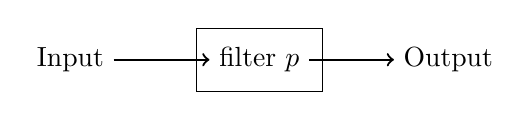
\begin{tikzpicture}[scale=0.8]
      \draw (2, 0) rectangle (4, 1) node (filter) [pos=.5] {filter $p$};
      \draw (0, .5) node (in) {Input}
            (6, .5) node (out) {Output};
      \draw[thick, ->] (in) edge (filter)
                       (filter) edge (out);
      \end{tikzpicture} \\
   \caption{Input: $[x_1, x_2, ..., x_n]$, Output: $[x_1', x_2', ..., x_m']$. and $\forall x_i' \Rightarrow p(x_i')$.}
   \label{fig:filter}
\end{figure}

Different from $find$, \textit{filter} returns empty list instead of \textit{Nothing} when no element satisfies the predicate.

\be
\begin{array}{rcl}
filter\ p\ [\ ] & = & [\ ] \\
filter\ p\ (x \cons xs) & = & \begin{cases}
  (p\ x): & x : filter\ p\ xs \\
  \text{otherwise}: & filter\ p\ xs \\
  \end{cases}
\end{array}
\ee

This definition builds the result from right. For iterative implementation, the performance will drop to $O(n^2)$ if build the result with \textproc{Append}. If change to \textproc{Cons}, then the order is reversed. We can further reverse it back in linear time (see the exercise).

\begin{algorithmic}[1]
\Function{Filter}{$p, X$}
  \State $X' \gets$ NIL
  \While{$X \neq$ NIL}
    \If{$p$(\Call{First}{$X$})}
      \State $X' \gets$ \textproc{Append}($X'$, \Call{First}{$X$}) \Comment{Linear time}
    \EndIf
    \State $L \gets$ \Call{Rest}{$X$}
  \EndWhile
\EndFunction
\end{algorithmic}

The nature to build result from right reminds us $foldr$. Define $f$ to test an element against the predicate, and prepend it to the result: $f\ p\ x\ as\ = \textbf{if}\ p\ x\ \textbf{then}\ x \cons as\ \textbf{else}\ as$. Use its Curried form to define $filter$:

\be
filter\ p = foldr\ (x\ as \mapsto f\ p\ x\ as)\ [\ ]
\ee

We can further simplify it (called $\eta$-conversion\cite{slpj-book-1987}) as:

\be
filter\ p = foldr\ (f\ p)\ [\ ]
\ee

Filter is a generic concept not only limit to list. We can apply a predicate to any traversable structure to extract things.

\index{List!matching} \index{List!prefix} \index{List!suffix} \index{List!infix}

Match is to find a pattern from some structure. Even if limit to list and string, there are still too many things to cover (chapter 14). The very basic problem is to test whether list $as$ exits in $bs$. There are two special cases: to test if $as$ is prefix or suffix of $bs$. The $span$ function actually finds the longest prefix under a given predicate. Similarly, we can compare each element between $as$ and $bs$. Define $as \subseteq bs$ if $as$ is prefix of $bs$:

\be
\begin{array}{rcl}
[\ ] \subseteq bs & = & True \\
(a \cons as) \subseteq [\ ] & = & False \\
(a \cons as) \subseteq (b \cons bs) & = & \begin{cases}
  a \neq b: & False \\
  a = b: & as \subseteq bs \\
  \end{cases}
\end{array}
\ee

Prefix testing takes linear time to scan the two lists. However, we can not do suffix testing in this way because it is expensive to align the right ends and scan backwards. This is different from array. Alternatively, we can reverse both lists in linear time, convert the problem to prefix testing:

\be
A \supseteq B = reverse(A) \subseteq reverse(B)
\ee

With $\subseteq$, we can test if a list is the sub-list of another one (infix testing). Define empty is infix of any list, we repeatedly apply prefix testing while traverse $B$:

\be
\begin{array}{rcl}
\textit{infix}?\ (a \cons as)\ [\ ] & = & False \\
\textit{infix}?\ A\ B & = & \begin{cases}
  A \subseteq B: & True \\
  \text{otherwise}: & \textit{infix}?\ A\ B' \\
  \end{cases}
\end{array}
\ee

Below is the iterative implementation:

\begin{algorithmic}[1]
\Function{Is-Infix}{$A, B$}
  \If{$A = $ NIL}
    \State \Return TRUE
  \EndIf
  \State $n \gets |A|$
  \While{$B \neq$ NIL and $n \leq |B|$}
    \If{$A \subseteq B$}
      \State \Return TRUE
    \EndIf
    \State $B \gets$ \Call{Rest}{$B$}
  \EndWhile
  \State \Return FALSE
\EndFunction
\end{algorithmic}

Because prefix testing runs in linear time, and is called in every loop. This implementation is bound to $O(nm)$ time, where $m, n$ are the length of the two lists. Symmetrically, we can enumerate all suffixes of $B$, and test if $A$ is prefix of any:

\be
\textit{infix}?\ A\ B = \exists S \in \textit{suffixes}\ B, A \subseteq S
\ee

Below example Haskell program implement infix testing with list comprehension:

\begin{Haskell}
isInfixOf a b = (not . null) [s | s <- tails b, a `isPrefixOf` s]
\end{Haskell}

Where \texttt{isPrefixOf} does the prefixing testing, \texttt{tails} generates all suffixes of a given list (exercise of this section).

\begin{Exercise}
\Question{Implement the linear time existence testing algorithm.}
\Question{Implement the iterative lookup algorithm.}
\Question{Implement the linear time filter algorithm through $reverse$.}
\Question{Implement the iterative prefix testing algorithm.}
\Question{Enumerate all suffixes of a list.}
\end{Exercise}

\section{zip and unzip}
\index{List!zip} \index{List!unzip}

The assoc list is a light weighted dictionary (map) for small data. It is easier than tree or heap based dictionary with the overhead of linear time lookup performance. In the `$n$-lights' puzzle, we build the assoc list as: $map\ (i \mapsto (i, 0))\ [1, 2, ..., n]$. We define a $zip$ function:

\be
\begin{array}{rcl}
zip\ as\ [\ ] & = & [\ ] \\
zip\ [\ ]\ bs & = & [\ ] \\
zip\ (a \cons as)\ (b \cons bs) & = & (a, b) : zip\ as\ bs \\
\end{array}
\ee

This implementation works when the two lists have different lengths. The result has the same length as the shorter one. We can even zip infinite lists (under lazy evaluation), for example\footnote{Or $zip\ (repeat\ 0)\ [1..n]$, where $repeat\ x = x : repeat\ x$.}: $zip\ [0, 0, ...]\ [1, 2, ..., n]$. For a list of words, we can index it as: $zip$ [1, 2, ...]\ [a, an, another, ...]. $zip$ builds the result from right. We can define it with $foldr$. It is bound to $O(m)$ time, where $m$ is the length of the shorter list. When implement the iterative $zip$, the performance will drop to quadratic if using \textproc{Append}, we can use \textproc{Cons} then reverse the result. However, this method can't handle two infinite lists. In imperative settings, we can reuse $A$ to hold the zip result (treat as transform every element to a pair).

\begin{algorithmic}[1]
\Function{Zip}{$A, B$}
  \State $C \gets$ NIL
  \While{$A \neq$ NIL and $B \neq$ NIL}
    \State $C \gets $ \textproc{Append}(C, (\Call{First}{$A$}, \Call{First}{$B$})) \Comment{Linear time}
    \State $A \gets$ \Call{Rest}{$A$}
    \State $B \gets$ \Call{Rest}{$B$}
  \EndWhile
  \State \Return $C$
\EndFunction
\end{algorithmic}

We can extend to $zip$ multiple lists. Some programming environments provide, \texttt{zip}, \texttt{zip3}, \texttt{zip4}, ... Sometimes, we want to apply a binary function to combine elements, but not just form a pair. For example, given a list of unit prices $[1.00, 0.80, 10.05, ...]$ for fruits: apple, orange, banana, ... and a list of quantities, like $[3, 1, 0, ...]$, meaning, buy 3 apples, 1 orange, 0 banana, ... Below program generates the payment list:

\[
\begin{array}{rcl}
pays\ us\ [\ ] & = & [\ ] \\
pays\ [\ ]\ qs & = & [\ ] \\
pays\ (u \cons us)\ (q \cons qs) & = & uq : pays\ us\ qs \\
\end{array}
\]

It has the same structure as $zip$ except using multiply but not `cons'. We can abstract the binary function as $f$:

\be
\begin{array}{rcl}
zipWith\ f\ as\ [\ ] & = & [\ ] \\
zipWith\ f\ [\ ]\ bs & = & [\ ] \\
zipWith\ f\ (a \cons as)\ (b \cons bs) & = & (f\ a\ b) : zipWith\ f\ as\ bs \\
\end{array}
\ee

For example, we can define the inner-product (or dot-product)\cite{wiki-dot-product} as: $A \cdot B = sum\ (zipWith\ (\cdot)\ A\ B)$, or define the infinite Fibonacci sequence with lazy evaluation:

\be
F = 0 : 1 : zipWith\ (+)\ F\ F'
\ee

Let $F$ be the infinite Fibonacci numbers, starts from 0 and 1. $F'$ drops the head. From the third number, every Fibonacci number is the sum of the corresponding numbers from $F$ and $F'$ at the same position. Below example program takes the first 15 Fibonacci numbers:

\begin{Haskell}
fib = 0 : 1 : zipWith (+) fib (tail fib)

take 15 fib
[0,1,1,2,3,5,8,13,21,34,55,89,144,233,377]
\end{Haskell}

$unzip$ is the inverse of $zip$. It converts a list of pairs to two separated lists. Define it with $foldr$ in Curried form:

\be
unzip = foldr\ ((a, b)\ (as, bs) \mapsto (a \cons as, b \cons bs))\ ([\ ], [\ ])
\ee

For the fruits example, given the unit price as an assoc list: $U$ = [(apple, 1.00), (orange, 0.80), (banana, 10.05), ...], the purchased quantity is also an assoc list: $Q$ = [(apple, 3), (orange, 1), (banana, 0), ...]. We extract the unit prices and the quantities, then compute their inner-product:

\be
pay = sum\ (zipWith\ (\cdot)\ snd(unzip\ U)\ snd(unzip\ Q))
\ee

$zip$ and $unzip$ are generic. We can expand to $zip$ two trees, where the nodes contain paired elements from both. When traverse a collection of elements, we can also use the generic $zip$ and $unzip$ to track the path. This is a method to mimic the `parent' reference in imperative implementation (last chapter of \cite{learn-haskell}).

List is fundamental to build more complex data structures and algorithms particularly in functional settings. We introduced elementary algorithms to construct, access, update, and transform list; how to search, filter data, and compute with list. Although most programming environments provide pre-defined tools and libraries to support list, we should not simply treat them as black-boxes. Rabhi and Lapalme introduce many functional algorithms about list\cite{algo-fp}. Haskell library provides detailed documentation about basic list algorithms. Bird gives good examples of folding\cite{fp-pearls}, and introduces about the {\em fold fusion law}.

\begin{Exercise}
\Question{Design the iota ($I$) operator for list, below are the use cases:
  \begin{itemize}
  \item $iota(..., n) = [1, 2, 3, ..., n]$;
  \item $iota(m, n) = [m, m + 1, m + 2, ..., n]$, where $m \leq n$;
  \item $iota(m, m+a, ..., n) = [m, m + a, m + 2a, ..., n]$;
  \item $iota(m, m, ...) = repeat(m) = [m, m, m, ...]$;
  \item $iota(m, ...) = [m, m + 1, m + 2, ... ]$.
  \end{itemize}
}

\Question{Implement the linear time imperative $zip$.}

\Question{Define $zip$ with $foldr$.}

\Question{For the fruits example, suppose the quantity assoc list only contains the items without zero quantity. i.e. instead of
\[
Q = [(apple, 3), (banana, 0), (orange, 1), ...]
\]
but
\[
Q = [(apple, 3), (orange, 1), ...]
\]
Write a program to calculate the total payment.}

\Question{Implement $lastAt$ with $zip$.} % lastAt k xs = (fst . last) $ zip xs  (drop k xs)

\Question{Write a program to remove the duplicated elements in a list while maintain the original order. For imperative implementation, the elements should be removed in-place. What is the complexity? How to simplify it with additional data structure?}

\Question{List can represent decimal non-negative integer. For example 1024 as list is $4 \rightarrow 2 \rightarrow 0 \rightarrow 1$. Generally, $n = d_m...d_2d_1$ can be represented as $d_1 \rightarrow d_2 \rightarrow ... \rightarrow d_m$. Given two numbers $a$, $b$ in list form. Realize arithmetic operations such as add and subtraction.}

\Question{In imperative settings, a circular linked-list is corrupted, that some node points back to previous one, as shown in figure \ref{fig:circular-list}. When traverse, it falls into infinite loops. Design an algorithm to detect if a list is circular. On top of that, improve it to find the node where loop starts (the node being pointed by two precedents).

\begin{center}
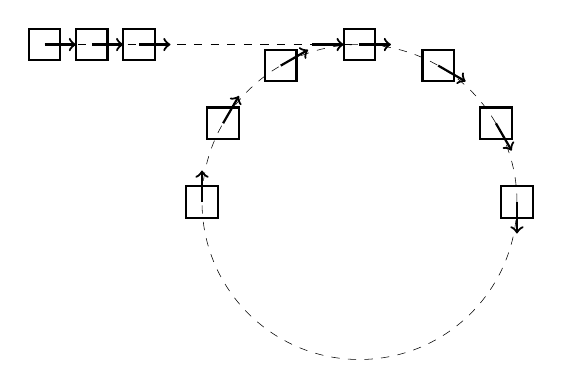
\begin{tikzpicture}[scale=2]
  % trace
  \draw[dashed, very thin] (-2cm, 1cm) -- (0, 1cm);
  \draw[dashed, very thin] (0,0) circle [radius=1cm];

  % leading nodes
  \foreach \x in {-2, -1.7, ..., -1.4} {
    \draw[thick] (\x cm, 1cm) +(-0.1, -0.1) rectangle ++(0.1, 0.1);
    \draw[thick, ->] (\x cm, 1cm) -- +(0.2, 0);
  }

  % cricular starting points
  \draw[thick, ->] (-0.3cm, 1cm) -- (-0.1cm, 1cm);

  % circular nodes
  \foreach \deg/\rot in {90/0, 60/-30, 30/-60, 0/-90, 180/90, 150/60, 120/30} {
    \draw[thick] (\deg : 1cm) +(-0.1, -0.1) rectangle ++(0.1, 0.1);
    \draw[thick, ->] (\deg : 1cm) -- +(\rot : 0.2);
  }
\end{tikzpicture}
\captionof{figure}{A circular linked-list}
\label{fig:circular-list}
\end{center}
}
\end{Exercise}

\ifx\wholebook\relax \else
\begin{thebibliography}{99}

\bibitem{fp-pearls}
Richard Bird. ``Pearls of Functional Algorithm Design''. Cambridge University Press; 1 edition (November 1, 2010). ISBN: 978-0521513388

\bibitem{slpj-book-1987}
Simon L. Peyton Jones. ``The Implementation of Functional Programming Languages''. Prentice-Hall International Series in Computer Since. Prentice Hall (May 1987). ISBN: 978-0134533339

\bibitem{moderncxx}
Andrei Alexandrescu. ``Modern C++ design: Generic Programming and Design Patterns Applied''. Addison Wesley February 01, 2001, ISBN 0-201-70431-5

\bibitem{mittype}
Benjamin C. Pierce. ``Types and Programming Languages''. The MIT Press, 2002. ISBN:0262162091

\bibitem{unplugged}
Xinyu LIU. ``Isomorphism -- mathematics of programming''. 2020. \url{https://github.com/liuxinyu95/unplugged}

\bibitem{SICP}
Harold Abelson, Gerald Jay Sussman, Julie Sussman. ``Structure and Interpretation of Computer Programs, 2nd Edition''. MIT Press, 1996, ISBN 0-262-51087-1

\bibitem{okasaki-book}
Chris Okasaki. ``Purely Functional Data Structures''. Cambridge university press, (July 1, 1999), ISBN-13: 978-0521663502

\bibitem{algo-fp}
Fethi Rabhi, Guy Lapalme. ``Algorithms: a functional programming approach''. Second edition. Addison-Wesley, 1999. ISBN: 0201-59604-0

\bibitem{learn-haskell}
Miran Lipovaca. ``Learn You a Haskell for Great Good! A Beginner's Guide''. No Starch Press; 1 edition April 2011, 400 pp. ISBN: 978-1-59327-283-8

\bibitem{erlang}
Joe Armstrong. ``Programming Erlang: Software for a Concurrent World''. Pragmatic Bookshelf; 1 edition (July 18, 2007). ISBN-13: 978-1934356005

\bibitem{wiki-tail-call}
Wikipedia. ``Tail call''. \url{https://en.wikipedia.org/wiki/Tail_call}

\bibitem{sgi-stl-transform}
SGI. ``transform''. \url{http://www.sgi.com/tech/stl/transform.html}

\bibitem{poj-drunk-jailer}
ACM/ICPC. ``The drunk jailer.'' Peking University judge online for ACM/ICPC. \url{http://poj.org/problem?id=1218}.

\bibitem{Haskell-wiki}
Haskell wiki. ``Haskell programming tips''. 4.4 Choose the appropriate fold. \url{http://www.haskell.org/haskellwiki/Haskell_programming_tips}

\bibitem{wiki-dot-product}
Wikipedia. ``Dot product''. \url{https://en.wikipedia.org/wiki/Dot_product}

\end{thebibliography}

\expandafter\enddocument
\fi
